\documentclass{article}
\usepackage{graphicx}

\begin{document}

\title{Introduction to \LaTeX{}}
\author{Author's Name}

\maketitle

\begin{figure}
    \centering
    \includegraphics[width= 0.3\textwidth]{DataPP/ResultsDataJetPt40_Dptmin4_Dptmax20_jetetamin0_jetetamax20_isPP1_Rindex0_indexBkg0.pdf}
    \includegraphics[width= 0.3\textwidth]{DataPP/ResultsDataJetPt40_Dptmin4_Dptmax20_jetetamin0_jetetamax20_isPP1_Rindex1_indexBkg0.pdf}
    \includegraphics[width= 0.3\textwidth]{DataPP/ResultsDataJetPt40_Dptmin4_Dptmax20_jetetamin0_jetetamax20_isPP1_Rindex2_indexBkg0.pdf}
    \includegraphics[width= 0.3\textwidth]{DataPP/ResultsDataJetPt40_Dptmin20_Dptmax999_jetetamin0_jetetamax20_isPP1_Rindex0_indexBkg0.pdf}
    \includegraphics[width= 0.3\textwidth]{DataPP/ResultsDataJetPt40_Dptmin20_Dptmax999_jetetamin0_jetetamax20_isPP1_Rindex1_indexBkg0.pdf}
    \includegraphics[width= 0.3\textwidth]{DataPP/ResultsDataJetPt40_Dptmin20_Dptmax999_jetetamin0_jetetamax20_isPP1_Rindex2_indexBkg0.pdf}
    \caption{proton proton data, Jet40 results, 4$<p_{T}<$20 GeV/c (top), $p_{T}>$20 GeV/c (bottom) }
    \label{simulationfigure}
\end{figure}


\begin{figure}
    \centering
    \includegraphics[width= 0.3\textwidth]{DataPP/ResultsDataJetPt60_Dptmin4_Dptmax20_jetetamin0_jetetamax20_isPP1_Rindex0_indexBkg0.pdf}
    \includegraphics[width= 0.3\textwidth]{DataPP/ResultsDataJetPt60_Dptmin4_Dptmax20_jetetamin0_jetetamax20_isPP1_Rindex1_indexBkg0.pdf}
    \includegraphics[width= 0.3\textwidth]{DataPP/ResultsDataJetPt60_Dptmin4_Dptmax20_jetetamin0_jetetamax20_isPP1_Rindex2_indexBkg0.pdf}
    \includegraphics[width= 0.3\textwidth]{DataPP/ResultsDataJetPt60_Dptmin20_Dptmax999_jetetamin0_jetetamax20_isPP1_Rindex0_indexBkg0.pdf}
    \includegraphics[width= 0.3\textwidth]{DataPP/ResultsDataJetPt60_Dptmin20_Dptmax999_jetetamin0_jetetamax20_isPP1_Rindex1_indexBkg0.pdf}
    \includegraphics[width= 0.3\textwidth]{DataPP/ResultsDataJetPt60_Dptmin20_Dptmax999_jetetamin0_jetetamax20_isPP1_Rindex2_indexBkg0.pdf}
    \caption{proton proton data, Jet60 results, 4$<p_{T}<$20 GeV/c (top), $p_{T}>$20 GeV/c (bottom) }
    \label{simulationfigure}
\end{figure}


\begin{figure}
    \centering
    \includegraphics[width= 0.3\textwidth]{DataPP/ResultsDataJetPt80_Dptmin4_Dptmax20_jetetamin0_jetetamax20_isPP1_Rindex0_indexBkg0.pdf}
    \includegraphics[width= 0.3\textwidth]{DataPP/ResultsDataJetPt80_Dptmin4_Dptmax20_jetetamin0_jetetamax20_isPP1_Rindex1_indexBkg0.pdf}
    \includegraphics[width= 0.3\textwidth]{DataPP/ResultsDataJetPt80_Dptmin4_Dptmax20_jetetamin0_jetetamax20_isPP1_Rindex2_indexBkg0.pdf}
    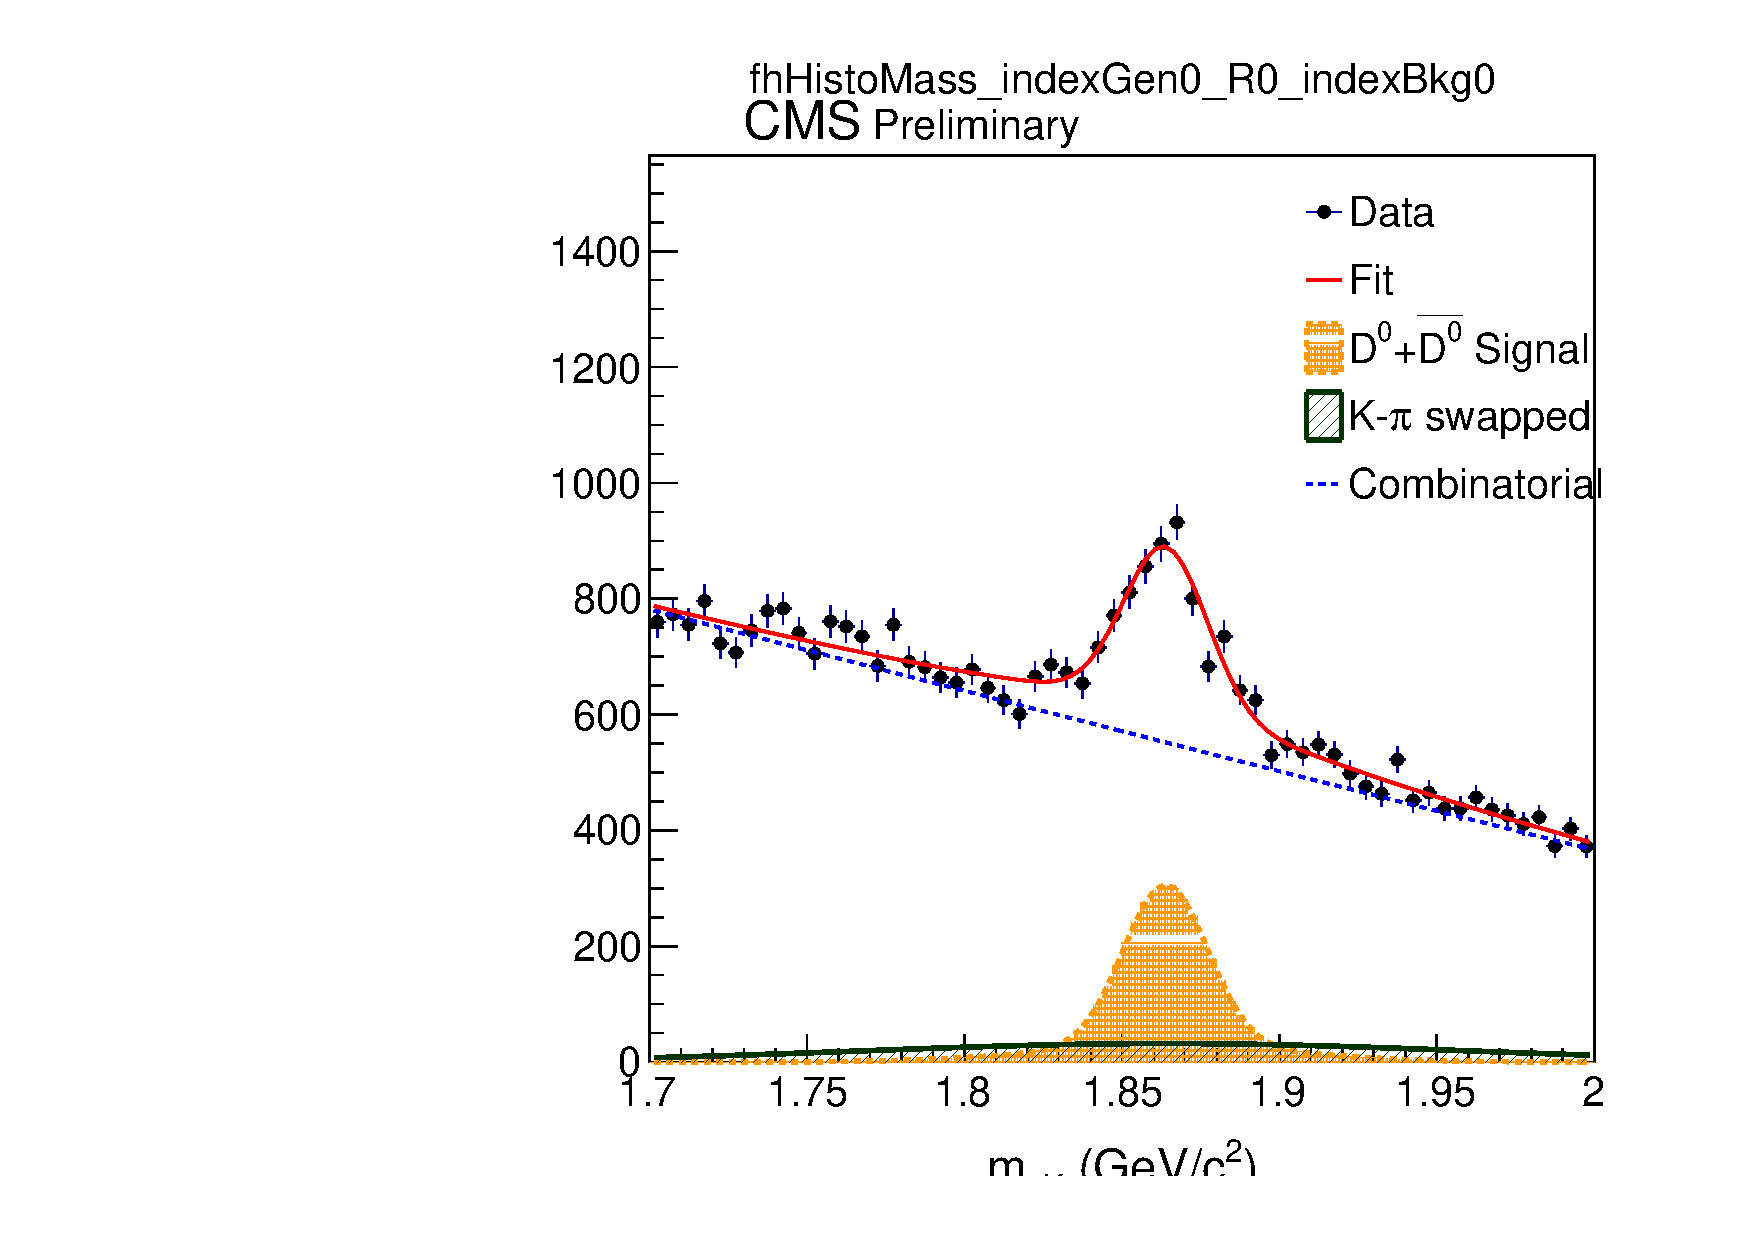
\includegraphics[width= 0.3\textwidth]{DataPP/ResultsDataJetPt80_Dptmin20_Dptmax999_jetetamin0_jetetamax20_isPP1_Rindex0_indexBkg0.pdf}
    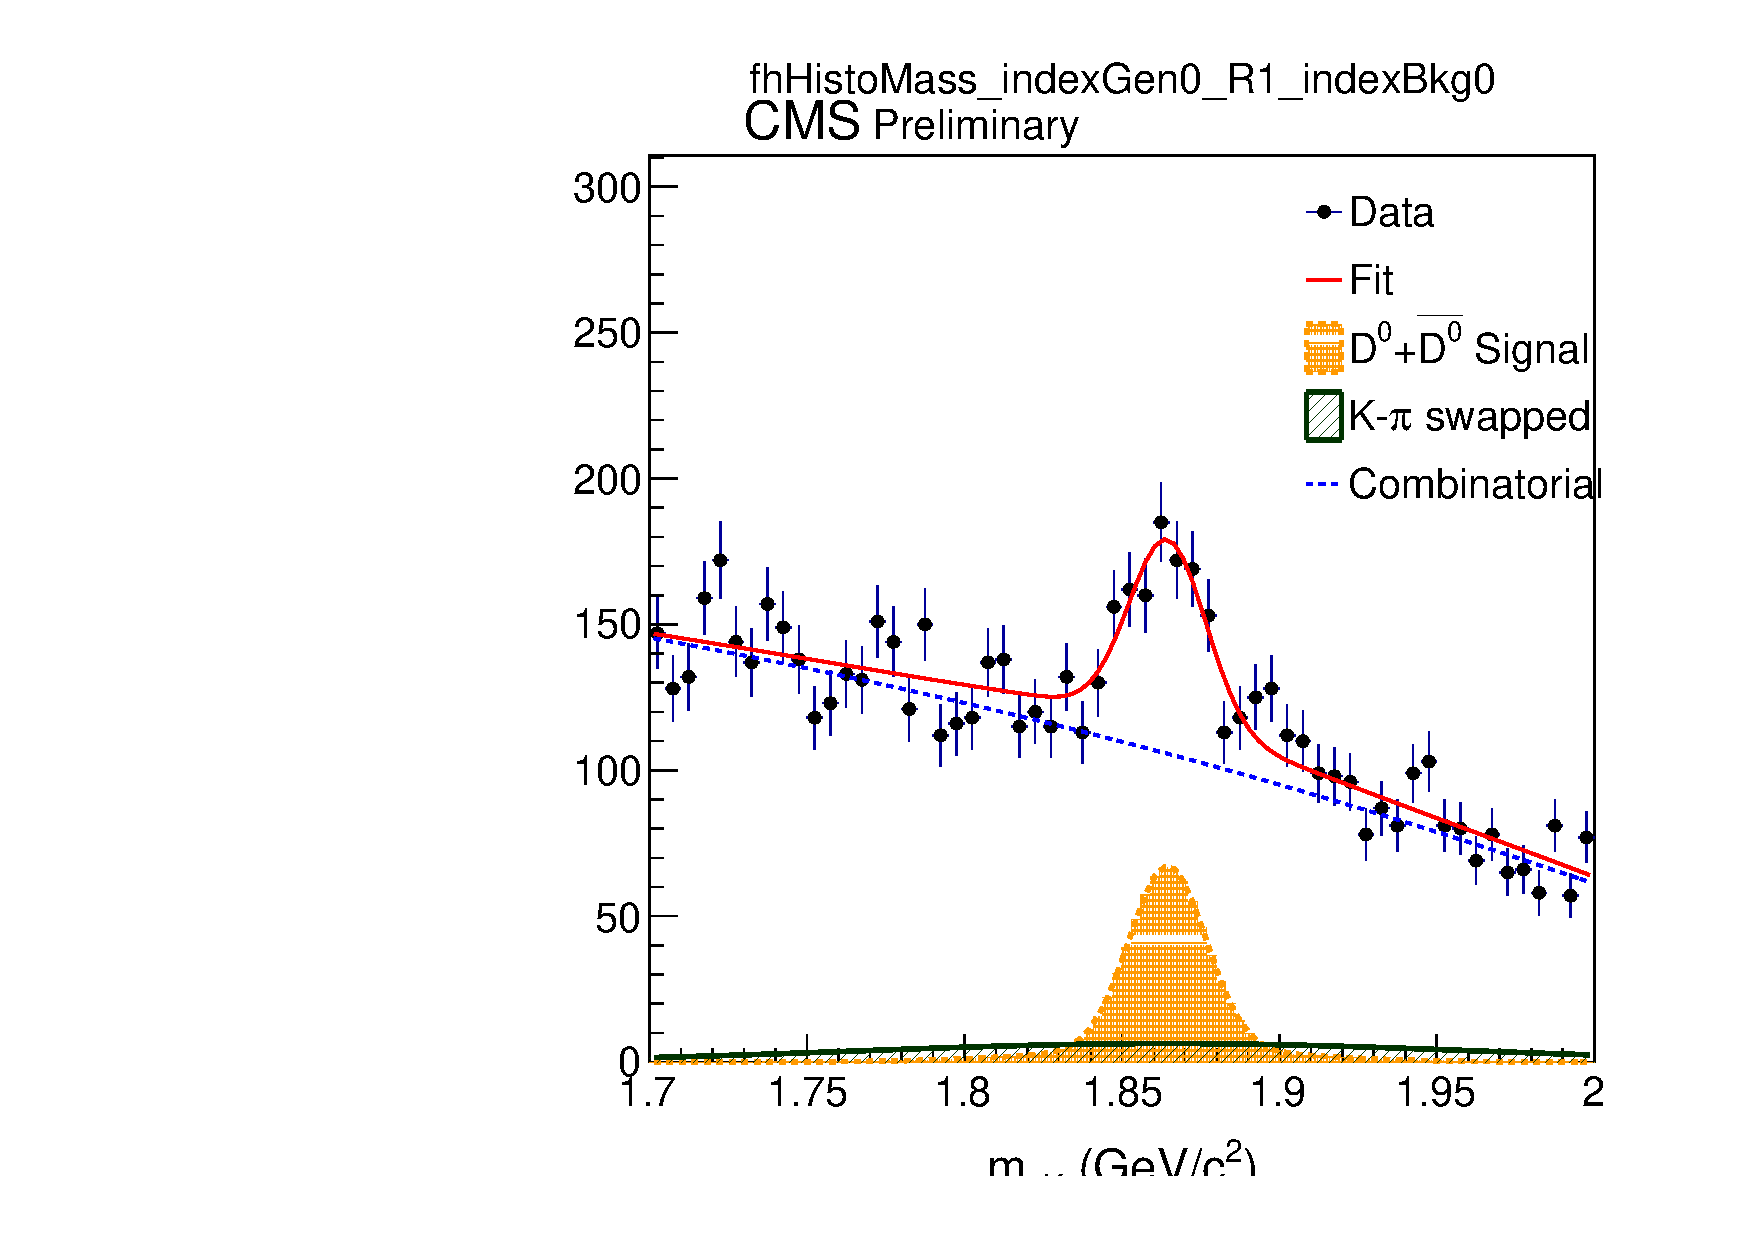
\includegraphics[width= 0.3\textwidth]{DataPP/ResultsDataJetPt80_Dptmin20_Dptmax999_jetetamin0_jetetamax20_isPP1_Rindex1_indexBkg0.pdf}
    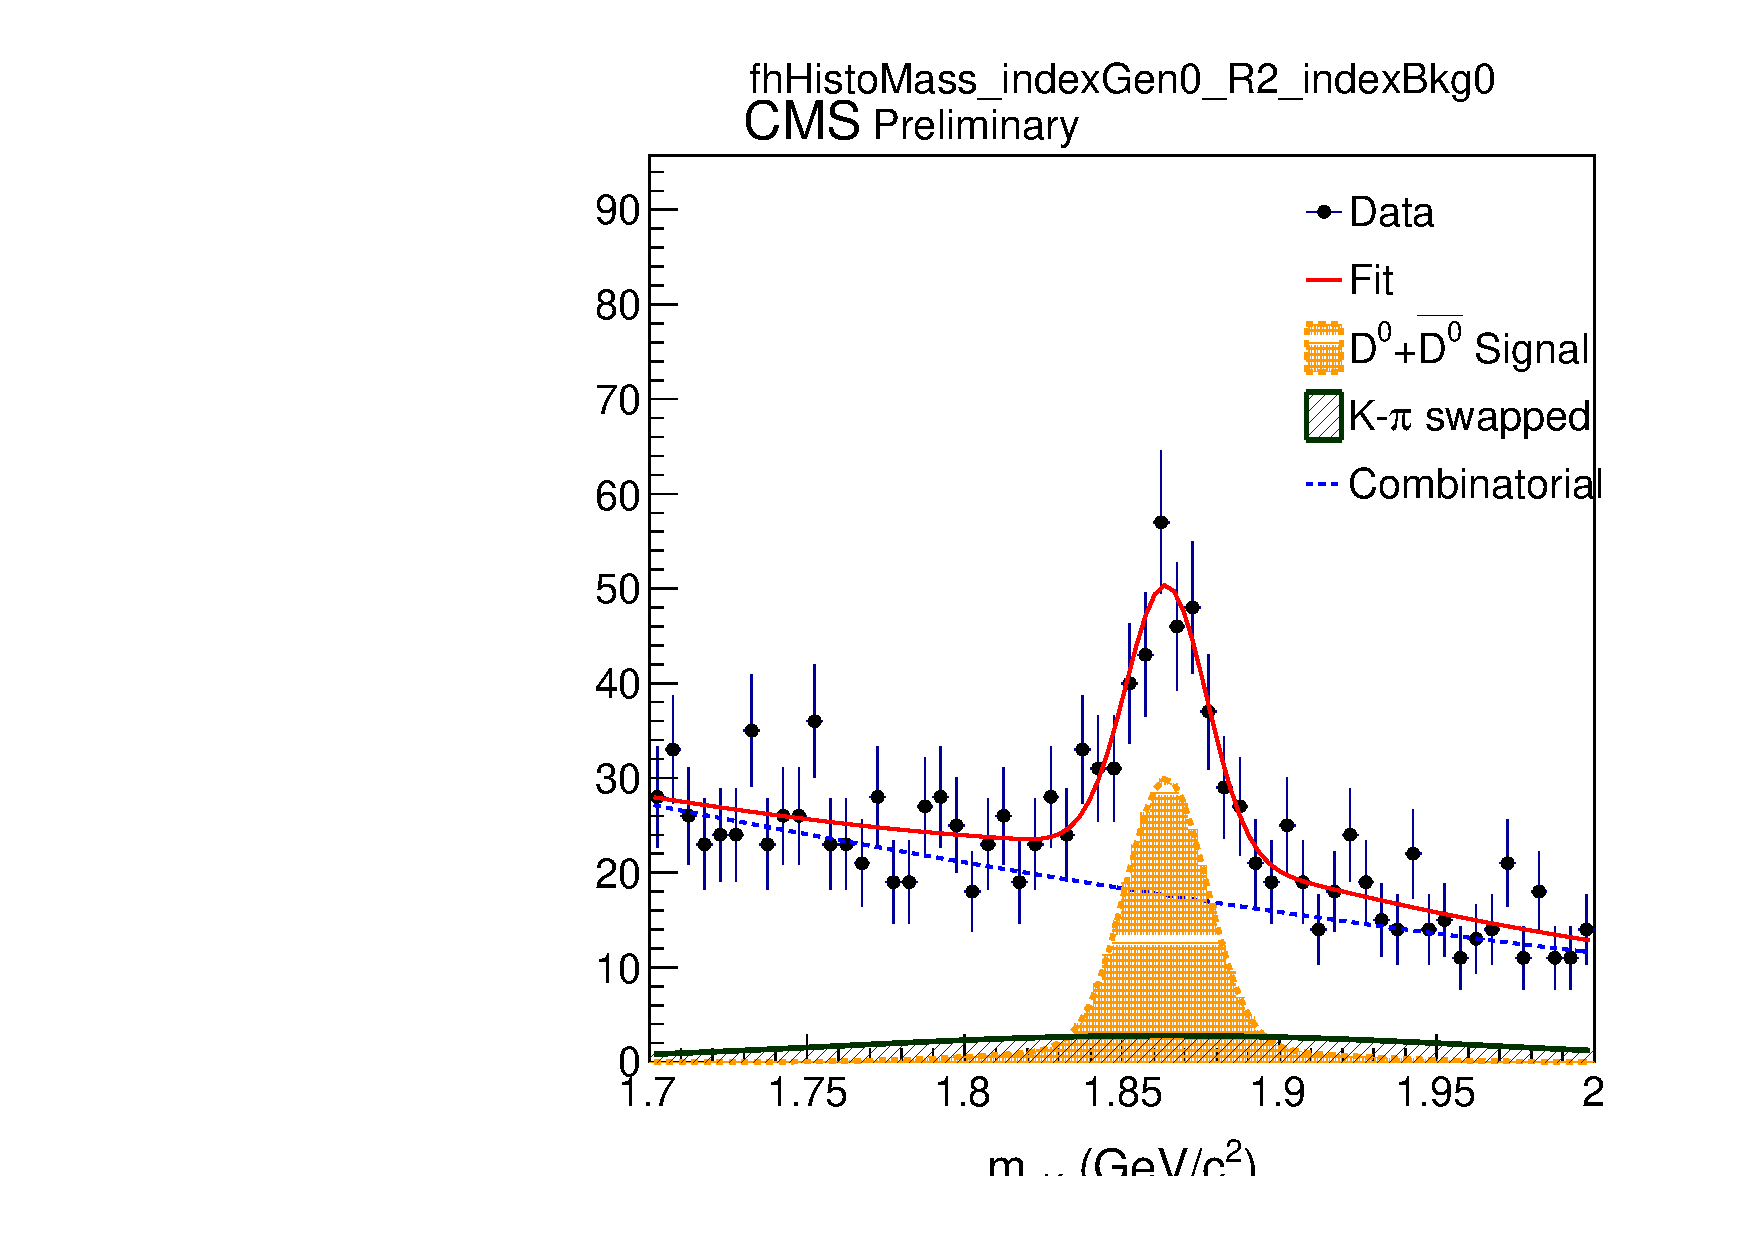
\includegraphics[width= 0.3\textwidth]{DataPP/ResultsDataJetPt80_Dptmin20_Dptmax999_jetetamin0_jetetamax20_isPP1_Rindex2_indexBkg0.pdf}
    \caption{proton proton data, Jet80 results, 4$<p_{T}<$20 GeV/c (top), $p_{T}>$20 GeV/c (bottom) }
    \label{simulationfigure}
\end{figure}


\begin{figure}
    \centering
    \includegraphics[width= 0.3\textwidth]{DataPbPb/ResultsDataJetPt40_Dptmin4_Dptmax20_jetetamin0_jetetamax20_isPP0_Rindex0_indexBkg0.pdf}
    \includegraphics[width= 0.3\textwidth]{DataPbPb/ResultsDataJetPt40_Dptmin4_Dptmax20_jetetamin0_jetetamax20_isPP0_Rindex1_indexBkg0.pdf}
    \includegraphics[width= 0.3\textwidth]{DataPbPb/ResultsDataJetPt40_Dptmin4_Dptmax20_jetetamin0_jetetamax20_isPP0_Rindex2_indexBkg0.pdf}
    \includegraphics[width= 0.3\textwidth]{DataPbPb/ResultsDataJetPt40_Dptmin20_Dptmax999_jetetamin0_jetetamax20_isPP0_Rindex0_indexBkg0.pdf}
    \includegraphics[width= 0.3\textwidth]{DataPbPb/ResultsDataJetPt40_Dptmin20_Dptmax999_jetetamin0_jetetamax20_isPP0_Rindex1_indexBkg0.pdf}
    \includegraphics[width= 0.3\textwidth]{DataPbPb/ResultsDataJetPt40_Dptmin20_Dptmax999_jetetamin0_jetetamax20_isPP0_Rindex2_indexBkg0.pdf}
    \caption{PbPb data, Jet40 results, 4$<p_{T}<$20 GeV/c (top), $p_{T}>$20 GeV/c (bottom) }
    \label{simulationfigure}
\end{figure}

\begin{figure}
    \centering
    \includegraphics[width= 0.3\textwidth]{DataPbPb/ResultsDataJetPt60_Dptmin4_Dptmax20_jetetamin0_jetetamax20_isPP0_Rindex0_indexBkg0.pdf}
    \includegraphics[width= 0.3\textwidth]{DataPbPb/ResultsDataJetPt60_Dptmin4_Dptmax20_jetetamin0_jetetamax20_isPP0_Rindex1_indexBkg0.pdf}
    \includegraphics[width= 0.3\textwidth]{DataPbPb/ResultsDataJetPt60_Dptmin4_Dptmax20_jetetamin0_jetetamax20_isPP0_Rindex2_indexBkg0.pdf}
    \includegraphics[width= 0.3\textwidth]{DataPbPb/ResultsDataJetPt60_Dptmin20_Dptmax999_jetetamin0_jetetamax20_isPP0_Rindex0_indexBkg0.pdf}
    \includegraphics[width= 0.3\textwidth]{DataPbPb/ResultsDataJetPt60_Dptmin20_Dptmax999_jetetamin0_jetetamax20_isPP0_Rindex1_indexBkg0.pdf}
    \includegraphics[width= 0.3\textwidth]{DataPbPb/ResultsDataJetPt60_Dptmin20_Dptmax999_jetetamin0_jetetamax20_isPP0_Rindex2_indexBkg0.pdf}
    \caption{PbPb data, Jet60 results, 4$<p_{T}<$20 GeV/c (top), $p_{T}>$20 GeV/c (bottom) }
    \label{simulationfigure}
\end{figure}


\begin{figure}
    \centering
    \includegraphics[width= 0.3\textwidth]{DataPbPb/ResultsDataJetPt80_Dptmin4_Dptmax20_jetetamin0_jetetamax20_isPP0_Rindex0_indexBkg0.pdf}
    \includegraphics[width= 0.3\textwidth]{DataPbPb/ResultsDataJetPt80_Dptmin4_Dptmax20_jetetamin0_jetetamax20_isPP0_Rindex1_indexBkg0.pdf}
    \includegraphics[width= 0.3\textwidth]{DataPbPb/ResultsDataJetPt80_Dptmin4_Dptmax20_jetetamin0_jetetamax20_isPP0_Rindex2_indexBkg0.pdf}
    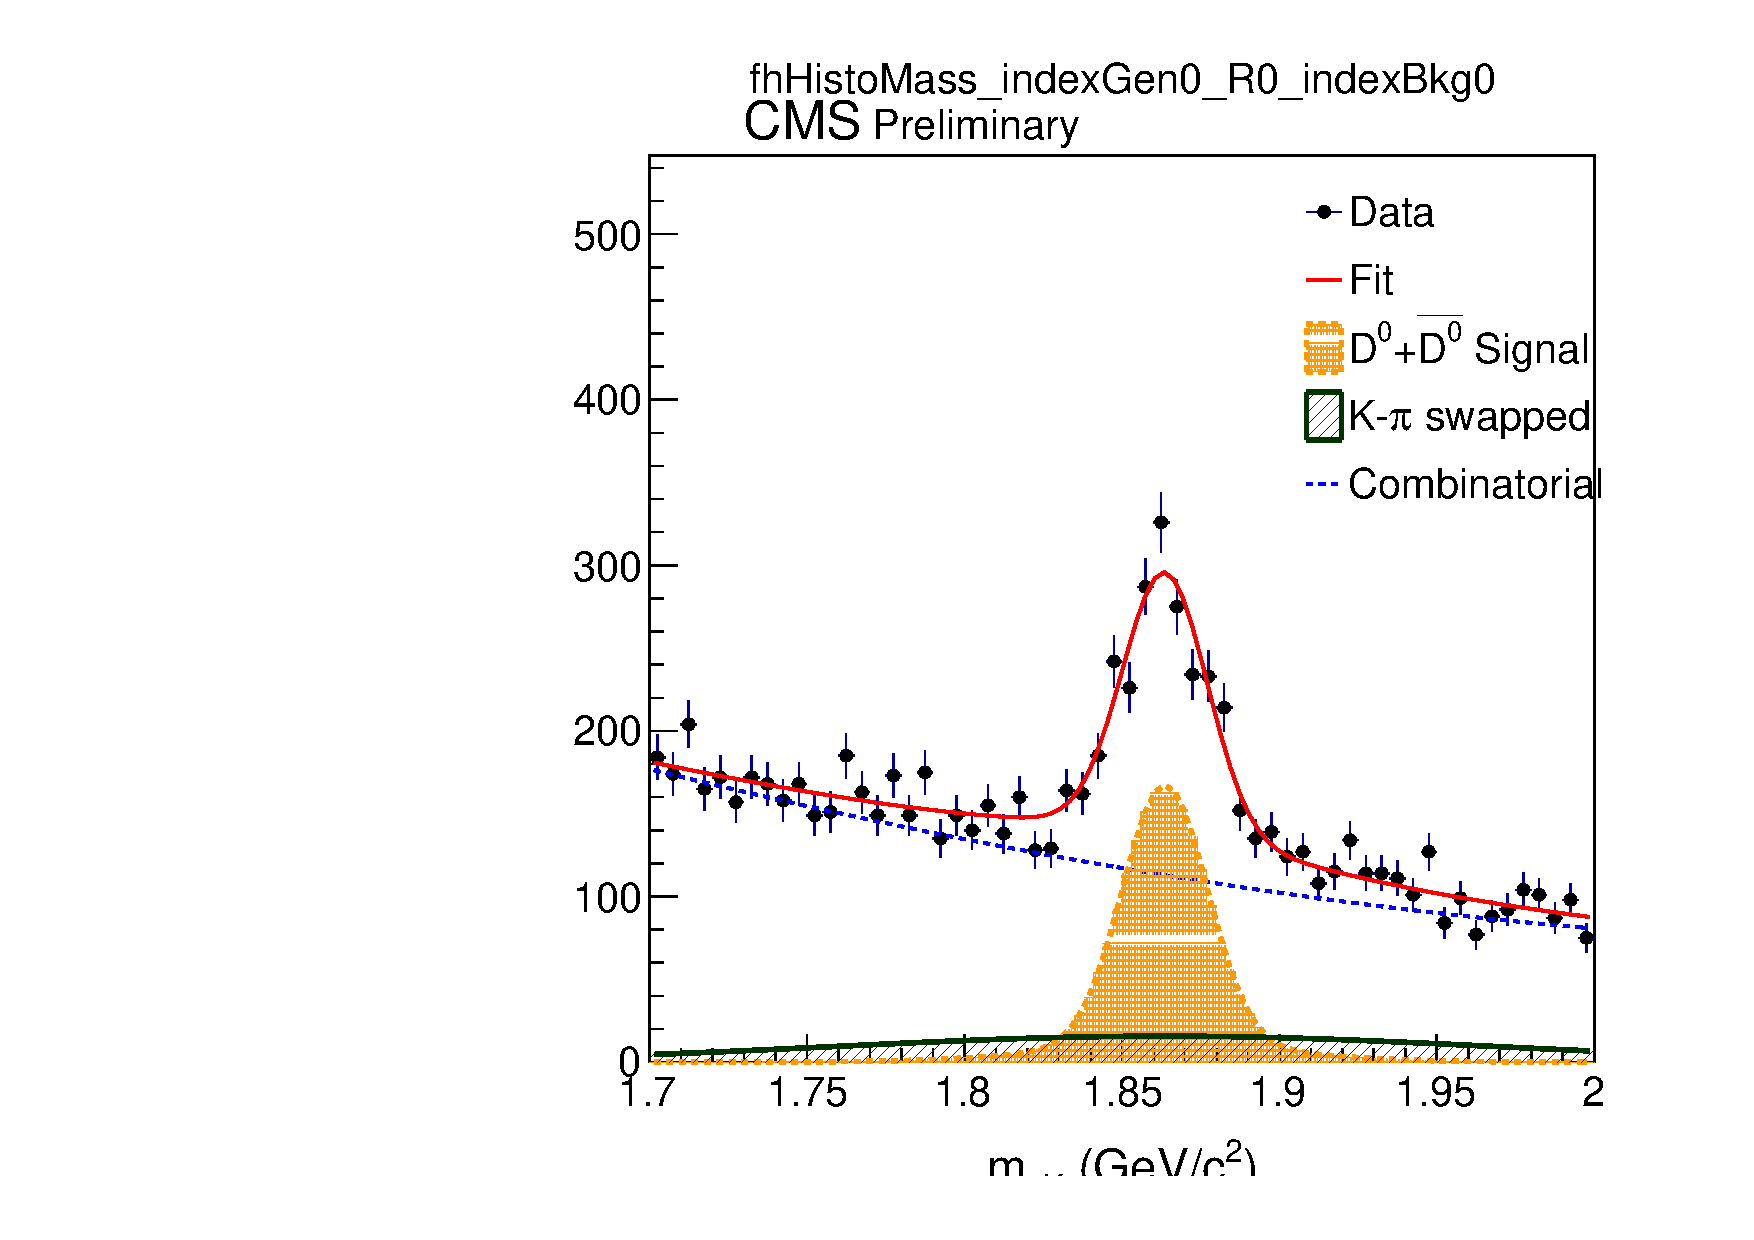
\includegraphics[width= 0.3\textwidth]{DataPbPb/ResultsDataJetPt80_Dptmin20_Dptmax999_jetetamin0_jetetamax20_isPP0_Rindex0_indexBkg0.pdf}
    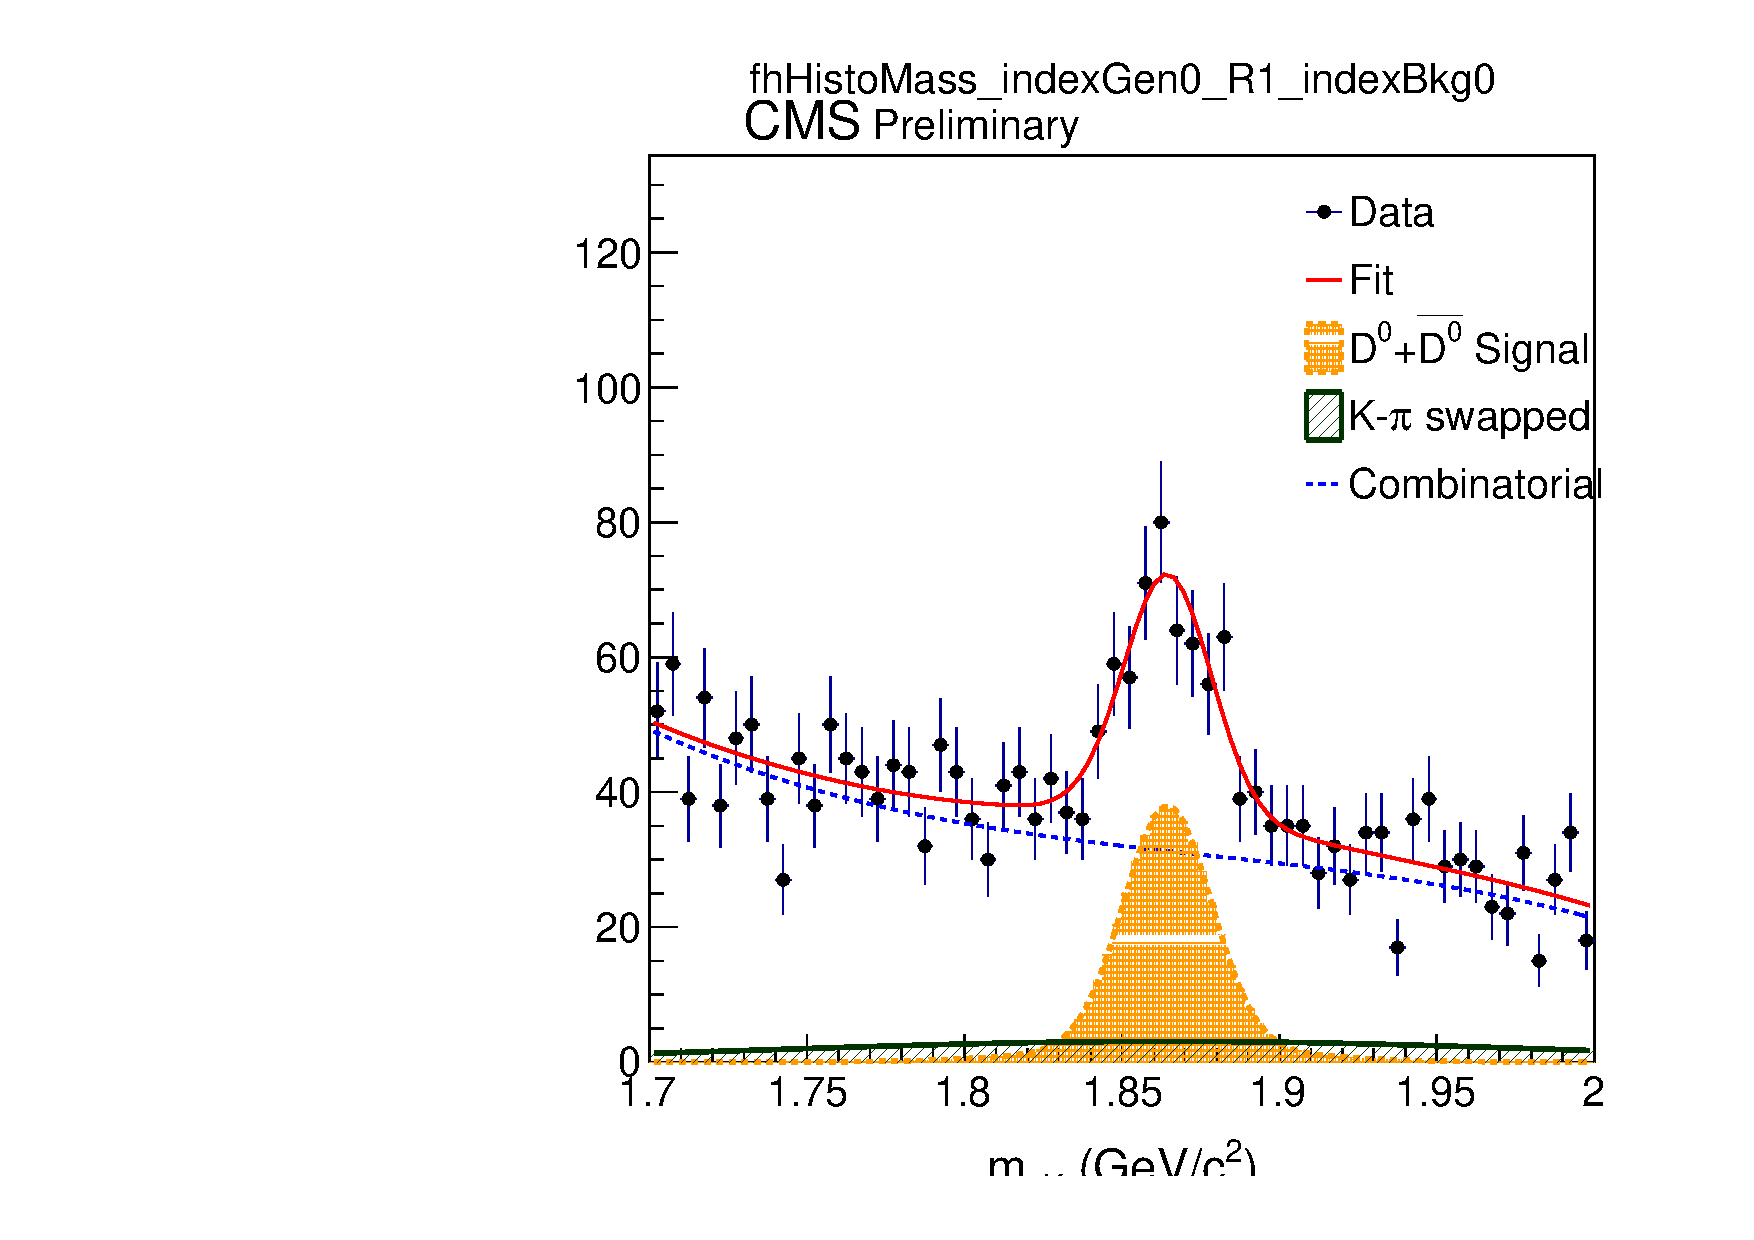
\includegraphics[width= 0.3\textwidth]{DataPbPb/ResultsDataJetPt80_Dptmin20_Dptmax999_jetetamin0_jetetamax20_isPP0_Rindex1_indexBkg0.pdf}
    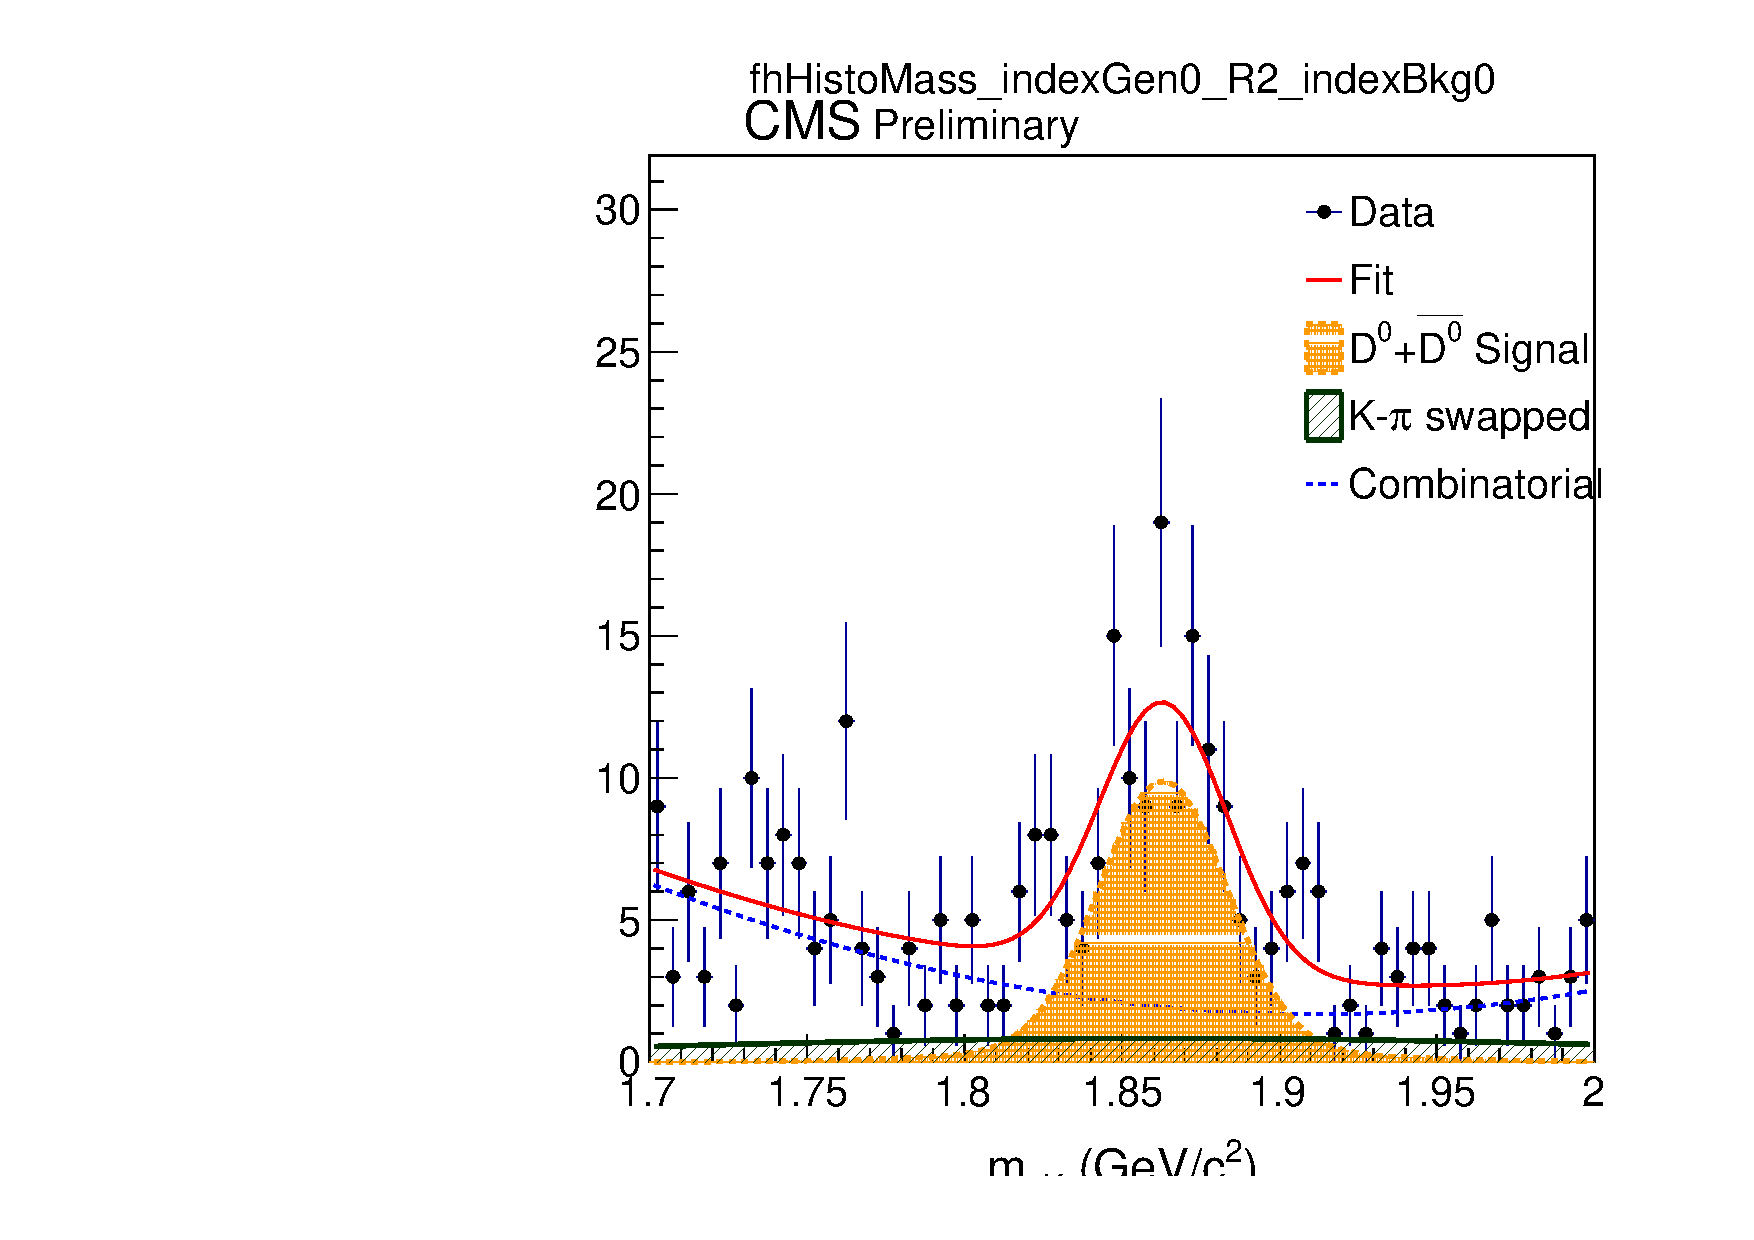
\includegraphics[width= 0.3\textwidth]{DataPbPb/ResultsDataJetPt80_Dptmin20_Dptmax999_jetetamin0_jetetamax20_isPP0_Rindex2_indexBkg0.pdf}
    \caption{PbPb data, Jet80 results, 4$<p_{T}<$20 GeV/c (top), $p_{T}>$20 GeV/c (bottom) }
    \label{simulationfigure}
\end{figure}

\end{document}
